%
% Chapter 5
%
\chapter {Analysis Framework}

The strategy we use to analyze Shor's integer factorization algorithm is very similar to the one proposed by Soeken et al.\cite{ResourceEstimationFramework_Soeken_2021}. The overview of the process is the following:
\begin{enumerate}
    \item Implement the quantum algorithm using a high-level programming language.
    \item Verify the correctness of the implementation by executing the algorithm in a full state simulator.
    \item Use, extend and build tools that can use the high-level algorithm implementation to estimate the amount of logical resources the algorithm requires depeding on its input size.
    \begin{enumerate}
        \item As part of logical resources estimation, consider the effects of introducing error-corrected qubits and fault-tolerant quantum gates on the amount of required resources.
    \end{enumerate}
    \item For each physical platform do the following:
    \begin{enumerate}
        \item Create a tool that uses platform specific parameters to calculate the amount of physical qubits, physical gates, and runtime required to run the algorithm.
        \item Analyze the data produced by the tool to determine the following:
        \begin{enumerate}
            \item The maximum input size for the algorithm to run on a real NISQ device.
            \item The characteristics that a device should have to run the algorithm for a specific input size, and determine what would be the runtime.
        \end{enumerate}
    \end{enumerate}
    \item Compare the results obtained for each physical platform.
\end{enumerate}

\section{Layered Architecture for Quantum Computing}

As a basis for the analysis, we will use a layered architecture model like the one proposed by N. Cody Jones et al.\cite{LayeredArchitectureForQuantum_2012}. Figure \ref{fig:LayeredArchitectureForQuantum} shows the five different layers of the architecture.

\begin{figure}[h!]
    \centering
    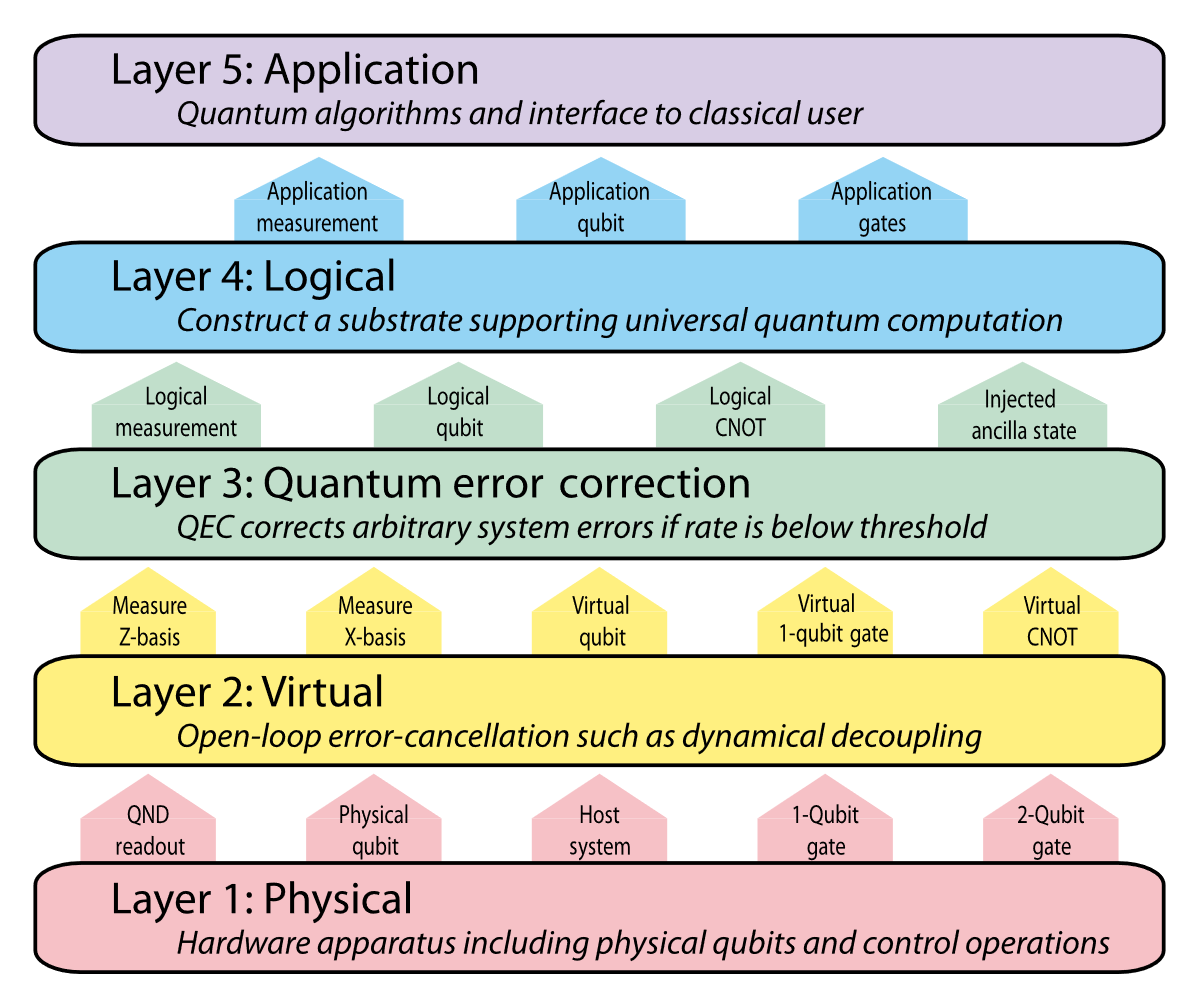
\includegraphics[scale=.35]{images/Framework-LayeredArchitecture.png}
    \caption{Layered architecture for quantum computing \cite{LayeredArchitectureForQuantum_2012}}
    \label{fig:LayeredArchitectureForQuantum}
\end{figure}

Briefly describing each layer:
\begin{enumerate}
    \item Physical: Consists of the physical qubits and the apparatus needed to manipulate them. At this layer, the gates that are native to the physical platform are the ones used for qubit manipulation.
    \item Virtual: Provides the interface to interact with the hardware such that the specifics of controlling it are abstracted away.
    \item Quantum error correction: Implements logical qubit encoding and fault-tolerant operations.
    \item Logical: Tools that allow the development of quantum algorithms at a higher level of abstraction. This layer exposes higher level gates that are decomposed into fault-tolerant sequences of native gates. Programming languages, frameworks and compilers belong to this layer.
    \item Application: Quantum algorithms like Shor's or Grover's implemented on top of the logical layer.
\end{enumerate}

The main advatage of a layered architecture like this one is modularity. Since each layer encapsulates its functionalities, the internal implementation of each layer can be changed as requirements and technology evolve. For example, the quantum error correcting code in the third layer can be changed depending on what works best for a specific physical platform.

\section{Q\# and the Quantum Development Kit (QDK)}

Microsoft's Quantum Development Kit (QDK)\cite{MicrosoftQuantumDevelopmentKit} is a set of tools for quantum application development. It includes Q\#, a high-level programming language, different quantum simulators and libraries that are useful for development and verification of quantum algorithms.

Quantum simulators are software programs that run on classical computers and act as the target machine for a Q\# program, making it possible to run and test quantum programs in an environment that handles qubits and operations that act on them\cite{QDKSimulators}. Each type of quantum simulator can provide different implementations of quantum primitive operations such as Hadamard, Pauli-X, Pauli-Y, Pauli-Z and CNOT. The ones we take advatage of are:
\begin{itemize}
    \item Full-state simulator: Runs quantum algorithms by tracking the full quantum state vector. It is limited to ~30 qubits.
    \item Resources estimator: Performs a top level analysis of the resources needed to run a quantum algorithm.
    \item Trace-based resource estimator: Runs advanced analysis of resources consumptions for the algorithm's entire call-graph.
\end{itemize}

Using Q\# and the QDK allows the algorithm implementation to remain constant even when the way it is executed changes, which is incredibly useful to verify the correctness of the implementation and to have confidence on the results it yields.

Additionally, the QDK supports the implementation of custom simulators that can be used to run Q\# programs. We leverage this capability and implement custom simulators that make calculations based on additional parameters.

\section{Command line application for verification and resources estimation}

In order to facilitate the verification of the correctness of the algorithm implementation and the calculation of resources making different assumptions, we developed a command line application that integrates the quantum algorithm implementation with both out-of-the-box QDK simulators and custom simulators. This way we can do the analysis from a single place.

Source code of a working version can be found in \href{https://github.com/cesarzc/uw-master-in-physics-project}{GitHub}.
